I en vanlig SR flip-flop er oppførselen uspesifisert for to høye input.
JK flip-flop løser problemet ved å bestemme at to høye input betyr flip.
Hva enn som var på output blir motsatt av hva det var.
\begin{figure}[H]
  \caption{JK flip-flop}
  \centering
    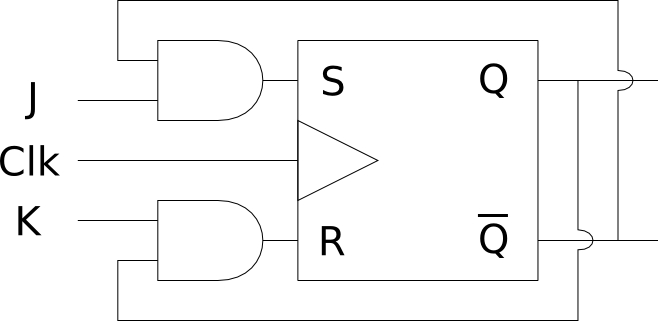
\includegraphics[width=\textwidth]{./img/jk}
\end{figure}
Sannhetstabellen til en JK flip-flop ser ut som følgende.
\begin{table}[H]
  \caption{JK sannhetstabell}
  \centering
  \begin{tabular}{c|c|c|c}
    J & K & Q & $\overline{Q}$ \\ \hline
    0 & 0 & Q & $\overline{Q}$ \\
    1 & 0 & 1 & 0 \\
    0 & 1 & 0 & 1 \\
    1 & 1 & $\overline{Q}$ & Q
  \end{tabular}
\end{table}
